% !TEX root = ../../../main.tex
% 来源：中学数学实验教材·第三册（高中数学）
% 章节：二次函数 / 和二次函数有关的课题
% 原始文件：5.tex，行 2084-2098
% 类型：tikz
% ---
    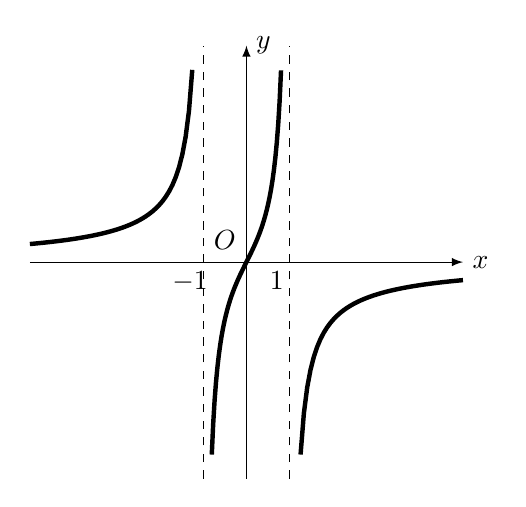
\begin{tikzpicture}[>=latex, scale=.55]
        \draw[->] (-5,0)--(5,0)node[right]{$x$};
      \draw[->] (0,-5)--(0,5)node[right]{$y$};  
      \foreach \x in {-1,1}
      {
          \node at (\x-.3,0)[below]{$\x$};
          \draw[dashed] (\x,-5)--(\x,5);
      }
      \draw [domain=-.8:.8, samples=50, ultra thick] plot(\x, {2*(\x/(1-\x*\x))});
      \draw [domain=-5:-1.25, samples=50, ultra thick] plot(\x, {2*(\x/(1-\x*\x))});
      \draw [domain=1.25:5, samples=50, ultra thick] plot(\x, {2*(\x/(1-\x*\x))});
    \node at (-.5,.5){$O$};
    

    \end{tikzpicture}
